\documentclass[11pt,a4paper,oneside]{report}             % Single-side
%\documentclass[11pt,a4paper,twoside,openright]{report}  % Duplex

\usepackage{ifxetex}
\usepackage{cmap}
\usepackage[T1]{fontenc}
\usepackage[utf8]{inputenc}
\usepackage{lmodern}

\usepackage[english,magyar]{babel} % Alapértelmezés szerint utoljára definiált nyelv lesz aktív, de később külön beállítjuk az aktív nyelvet.

\usepackage{amsfonts,amsmath,amssymb} % Mathematical symbols.
\usepackage[ruled,boxed,resetcount,linesnumbered]{algorithm2e} % For pseudocodes.
\usepackage{booktabs} % For publication quality tables for LaTeX
\usepackage{graphicx}
\usepackage{pdfpages}
\usepackage{multirow}
\usepackage{array}

%\usepackage{fancyhdr}
%\usepackage{lastpage}

\usepackage{anysize}
\usepackage{sectsty}
\usepackage{setspace}  % Ettol a tablazatok, abrak, labjegyzetek maradnak 1-es sorkozzel!

\usepackage[unicode]{hyperref} % For hyperlinks in the generated document. 

\usepackage{color}
\usepackage{listings} % For source code snippets.

\usepackage[amsmath,thmmarks]{ntheorem} % Theorem-like environments.

\usepackage[hang]{caption}

\newcommand{\selecthungarian}{
	\selectlanguage{magyar}
	\setlength{\parindent}{0em} % angol nyelvű dokumentumokban jellemző
	\setlength{\parskip}{0.5em} % angol nyelvű dokumentumokban jellemző
	\nonfrenchspacing
}

\newcommand{\selectenglish}{
	\selectlanguage{english}
	\setlength{\parindent}{2em} % angol nyelvű dokumentumokban jellemző
	\setlength{\parskip}{0em}   % angol nyelvű dokumentumokban jellemző
	\frenchspacing
	\renewcommand{\figureautorefname}{Figure}
	\renewcommand{\tableautorefname}{Table}
	\renewcommand{\partautorefname}{Part}
	\renewcommand{\chapterautorefname}{Chapter}
	\renewcommand{\sectionautorefname}{Section}
	\renewcommand{\subsectionautorefname}{Section}
	\renewcommand{\subsubsectionautorefname}{Section}
}


%--------------------------------------------------------------------------------------
% Main variables

%--------------------------------------------------------------------------------------
\newcommand{\vikszerzoVezeteknev}{Vincze}
\newcommand{\vikszerzoKeresztnev}{Balázs}
\newcommand{\vikkonzulensA}{Semeráth Oszkár} % Első konzulens neve
\newcommand{\vikkonzulensB}{Szombath István} % Második konzulens neve; hagyd üresen, ha egy konzulensed van.
\newcommand{\vikcim}{Peer-to-peer alapú számítógépes infrastruktúra kialakítása oktatási környezetben} % Cím
\newcommand{\viktanszek}{\bmemit} % Tanszék
\newcommand{\vikdoktipus}{\bsc} % Dokumentum típusa (\bsc, \msc)

%%--------------------------------------------------------------------------------------
% TDK-specifikus változók
%--------------------------------------------------------------------------------------
\newcommand{\tdkszerzoB}{Második Szerző} % Második szerző neve; hagyd üresen, ha egyedül í­rtad a TDK-t.
\newcommand{\tdkev}{2014} % A dolgozat írásának éve (pl. "2014") (Ez OTDK-nál eltérhet az aktuális évtől.)

% További adatok az OTDK címlaphoz (BME-s TDK-hoz nem kell kitölteni)
\newcommand{\tdkevfolyamA}{IV} % Első szerző évfolyama, római számmal (pl. IV).
\newcommand{\tdkevfolyamB}{III} % Második szerző évfolyama, római számmal (pl. III).
\newcommand{\tdkkonzulensbeosztasA}{egyetemi tanár} % Első konzulens beosztása (pl. egyetemi docens)
\newcommand{\tdkkonzulensbeosztasB}{doktorandusz} % Második konzulens beosztása (pl. egyetemi docens)

\newcommand{\szerzoMeta}{\vikszerzoVezeteknev{} \vikszerzoKeresztnev} % egy szerző esetén

%--------------------------------------------------------------------------------------
% Elnevezések
%--------------------------------------------------------------------------------------
\newcommand{\dolgozatnyelve}{
	\selectlanguage{magyar}
	\frenchspacing
}

\newcommand{\bme}{Budapesti Műszaki és Gazdaságtudományi Egyetem}
\newcommand{\vik}{Villamosmérnöki és Informatikai Kar}

\newcommand{\bmemit}{Méréstechnika és Információs Rendszerek Tanszék}

\newcommand{\keszitette}{Készítette}
\newcommand{\konzulens}{Konzulens}

\newcommand{\bsc}{Szakdolgozat}
\newcommand{\msc}{Diplomaterv}

\newcommand{\pelda}{Példa}
\newcommand{\definicio}{Definíció}
\newcommand{\tetel}{Tétel}

\newcommand{\bevezeto}{Bevezető}
\newcommand{\koszonetnyilvanitas}{Köszönetnyilvánítás}
\newcommand{\abrakjegyzeke}{Ábrák jegyzéke}
\newcommand{\tablazatokjegyzeke}{Táblázatok jegyzéke}
\newcommand{\irodalomjegyzek}{Irodalomjegyzék}
\newcommand{\fuggelek}{Függelék}

\newcommand{\szerzo}{\vikszerzoVezeteknev{} \vikszerzoKeresztnev}

\newcommand{\selectthesislanguage}{\selecthungarian}

\bibliographystyle{unsrt}

\def\lstlistingname{lista}
  % Beállítások magyar nyelvű dolgozathoz

%--------------------------------------------------------------------------------------
% Page layout setup
%--------------------------------------------------------------------------------------
% we need to redefine the pagestyle plain
% another possibility is to use the body of this command without \fancypagestyle
% and use \pagestyle{fancy} but in that case the special pages
% (like the ToC, the References, and the Chapter pages)remain in plane style

\pagestyle{plain}
\marginsize{35mm}{25mm}{15mm}{15mm}

\setcounter{secnumdepth}{0}
\sectionfont{\large\upshape\bfseries}
\setcounter{secnumdepth}{2}

\sloppy % Margón túllógó sorok tiltása.
\widowpenalty=10000 \clubpenalty=10000 %A fattyú- és árvasorok elkerülése
\def\hyph{-\penalty0\hskip0pt\relax} % Kötőjeles szavak elválasztásának engedélyezése


%--------------------------------------------------------------------------------------
% Setup hyperref package
%--------------------------------------------------------------------------------------
\hypersetup{
    bookmarks=true,            % show bookmarks bar?
    unicode=false,              % non-Latin characters in Acrobat's bookmarks
    pdftitle={\vikcim},        % title
    pdfauthor={\szerzoMeta},    % author
    pdfsubject={\vikdoktipus}, % subject of the document
    pdfcreator={\szerzoMeta},   % creator of the document
    pdfproducer={},    % producer of the document
    pdfkeywords={},    % list of keywords (separate then by comma)
    pdfnewwindow=true,         % links in new window
    colorlinks=true,           % false: boxed links; true: colored links
    linkcolor=black,           % color of internal links
    citecolor=black,           % color of links to bibliography
    filecolor=black,           % color of file links
    urlcolor=black             % color of external links
}


%--------------------------------------------------------------------------------------
% Set up listings
%--------------------------------------------------------------------------------------
\definecolor{lightgray}{rgb}{0.95,0.95,0.95}
\lstset{
	basicstyle=\scriptsize\ttfamily, % print whole listing small
	keywordstyle=\color{black}\bfseries, % bold black keywords
	identifierstyle=, % nothing happens
	commentstyle=\color{green}, % green comments
	stringstyle=\scriptsize,
	showstringspaces=false, % no special string spaces
	aboveskip=3pt,
	belowskip=3pt,
	backgroundcolor=\color{lightgray},
	columns=flexible,
	keepspaces=true,
	escapeinside={(*@}{@*)},
	captionpos=b,
	literate=*
		{á}{{\'a}}1	{é}{{\'e}}1	{í}{{\'i}}1	{ó}{{\'o}}1	{ö}{{\"o}}1	{ő}{{\H{o}}}1	{ú}{{\'u}}1	{ü}{{\"u}}1	{ű}{{\H{u}}}1
		{Á}{{\'A}}1	{É}{{\'E}}1	{Í}{{\'I}}1	{Ó}{{\'O}}1	{Ö}{{\"O}}1	{Ő}{{\H{O}}}1	{Ú}{{\'U}}1	{Ü}{{\"U}}1	{Ű}{{\H{U}}}1
}


%--------------------------------------------------------------------------------------
% Set up theorem-like environments
%--------------------------------------------------------------------------------------
% Using ntheorem package -- see http://www.math.washington.edu/tex-archive/macros/latex/contrib/ntheorem/ntheorem.pdf

\theoremstyle{plain}
\theoremseparator{.}
\newtheorem{example}{\pelda}

\theoremseparator{.}
%\theoremprework{\bigskip\hrule\medskip}
%\theorempostwork{\hrule\bigskip}
\theorembodyfont{\upshape}
\theoremsymbol{{\large \ensuremath{\centerdot}}}
\newtheorem{definition}{\definicio}

\theoremseparator{.}
%\theoremprework{\bigskip\hrule\medskip}
%\theorempostwork{\hrule\bigskip}
\newtheorem{theorem}{\tetel}


%--------------------------------------------------------------------------------------
% Some new commands and declarations
%--------------------------------------------------------------------------------------
\newcommand{\code}[1]{{\upshape\ttfamily\scriptsize\indent #1}}
\newcommand{\doi}[1]{DOI: \href{http://dx.doi.org/\detokenize{#1}}{\raggedright{\texttt{\detokenize{#1}}}}} % A hivatkozások közt így könnyebb DOI-t megadni.

\DeclareMathOperator*{\argmax}{arg\,max}
%\DeclareMathOperator*[1]{\floor}{arg\,max}
\DeclareMathOperator{\sign}{sgn}
\DeclareMathOperator{\rot}{rot}


%--------------------------------------------------------------------------------------
% Setup captions
%--------------------------------------------------------------------------------------
\captionsetup[figure]{
	width=.75\textwidth,
	aboveskip=10pt}

\renewcommand{\captionlabelfont}{\bf}
%\renewcommand{\captionfont}{\footnotesize\it}


%--------------------------------------------------------------------------------------
% Redefine reference style
%--------------------------------------------------------------------------------------
\newcommand{\figref}[1]{\ref{fig:#1}.}
\renewcommand{\eqref}[1]{(\ref{eq:#1})}
\newcommand{\listref}[1]{\ref{listing:#1}.}
\newcommand{\sectref}[1]{\ref{sect:#1}}
\newcommand{\tabref}[1]{\ref{tab:#1}.}


%--------------------------------------------------------------------------------------
% Hyphenation exceptions
%--------------------------------------------------------------------------------------
\hyphenation{Shakes-peare Mar-seilles ár-víz-tű-rő tü-kör-fú-ró-gép}


\author{\vikszerzo}
\title{\viktitle}

%--------------------------------------------------------------------------------------
% Table of contents and the main text
%--------------------------------------------------------------------------------------
\begin{document}

	%--------------------------------------------------------------------------------------
%	The title page
%--------------------------------------------------------------------------------------
\begin{titlepage}
\begin{center}

\includegraphics[width=60mm,keepaspectratio]{figures/bme_logo.pdf}\\
\vspace{0.3cm}
\textbf{\bme}\\
\textmd{\vik}\\
\textmd{\viktanszek}\\[5cm]

\vspace{0.4cm}
{\huge \bfseries \vikcim}\\[0.8cm]
\vspace{0.5cm}
\textsc{\Large \vikdoktipus}\\[4cm]

{
	\renewcommand{\arraystretch}{0.85}
	\begin{tabular}{cc}
	 \makebox[7cm]{\emph{\keszitette}} & \makebox[7cm]{\emph{\konzulens}} \\ \noalign{\smallskip}
	 \makebox[7cm]{\szerzo} & \makebox[7cm]{\vikkonzulensA} \\
	  & \makebox[7cm]{\vikkonzulensB} \\
	\end{tabular}
}

\vfill
{\large \today}
\end{center}
\end{titlepage}


		   % Szakdolgozat/Diplomaterv címlap

% Table of Contents
	\tableofcontents\vfill

% Declaration and Abstract
	\selectlanguage{magyar}
\pagenumbering{gobble}
%--------------------------------------------------------------------------------------
% Nyilatkozat
%--------------------------------------------------------------------------------------
\begin{center}
\large
\textbf{HALLGATÓI NYILATKOZAT}\\
\end{center}

Alulírott \emph{\vikszerzoVezeteknev{} \vikszerzoKeresztnev}, szigorló hallgató kijelentem, hogy ezt a szakdolgozatot/ diplomatervet \textcolor{blue}{(nem kívánt törlendő)} meg nem engedett segítség nélkül, saját magam készítettem, csak a megadott forrásokat (szakirodalom, eszközök stb.) használtam fel. Minden olyan részt, melyet szó szerint, vagy azonos értelemben, de átfogalmazva más forrásból átvettem, egyértelműen, a forrás megadásával megjelöltem.

Hozzájárulok, hogy a jelen munkám alapadatait (szerző(k), cím, angol és magyar nyelvű tartalmi kivonat, készítés éve, konzulens(ek) neve) a BME VIK nyilvánosan hozzáférhető elektronikus formában, a munka teljes szövegét pedig az egyetem belső hálózatán keresztül (vagy autentikált felhasználók számára) közzétegye. Kijelentem, hogy a benyújtott munka és annak elektronikus verziója megegyezik. Dékáni engedéllyel titkosított diplomatervek esetén a dolgozat szövege csak 3 év eltelte után válik hozzáférhetővé.

\begin{flushleft}
\vspace*{1cm}
Budapest, \today
\end{flushleft}

\begin{flushright}
 \vspace*{1cm}
 \makebox[7cm]{\rule{6cm}{.4pt}}\\
 \makebox[7cm]{\emph{\vikszerzoVezeteknev{} \vikszerzoKeresztnev}}\\
 \makebox[7cm]{hallgató}
\end{flushright}
\thispagestyle{empty}

\vfill
\clearpage
\thispagestyle{empty} % an empty page

\dolgozatnyelve
	\pagenumbering{roman}
\setcounter{page}{1}

%----------------------------------------------------------------------------
% Abstract in Hungarian
%----------------------------------------------------------------------------
\selecthungarian
\chapter*{Kivonat}\addcontentsline{toc}{chapter}{Kivonat}

Egy 40 gépből álló labor karbantartása komoly kihívást jelent, mivel minden tanórához különböző mérési környezet létrehozása szükséges.
Ezeket a környezeteket tipikusan virtuális gépekkel valósítjuk meg, amiknek szétosztását a laborban terítésnek nevezzük. A terítésére most egy Chaincast nevű megoldást használunk, ami abból áll, hogy a gépeket láncba kötjük és a láncon mennek végig a küldendő adatok. Ezáltal, ha bármelyik gépen hiba lép fel, akkor az adatátvitel meghiúsul és a terítést előlről kell kezdenünk. Továbbá, mivel minden tárgyhoz különbőző gépek kellenek (például csak az első három sor gépei), ezekhez a láncoknak különböző konfigurációja szükséges.

Dolgozatomnak célja, hogy egy olyan fájlterítési módszert dolgozzak ki, ami a terítés hibák esetén is sikeresen végrehajtható marad. Így a folyamat olyankor is sikeres lehet, amikor a korábbi módszer kudarcot vallott. Továbbá tetszőleges gépek kijelölhetőek minden laborhoz.

Dolgozatomban bemutatok egy új módszert a fájlok terítésére, ami a most használtnak a problémáit oldja meg, amellyel javítható az eljárás robusztussága és konfigurálhatósága. Bemutatok egy általam fejlesztett alkalmazást, ami Peer-to-Peer-alapon, ezen belül Bittorrent protokollt használva valósít meg fájlterítést, ahol a terítési feladatok egy könnyen használható modellen specifikálhatóak. Ismertetem a felhasznált technológiákat, a megértéshez szükséges háttérismereteket, majd bemutatom a tervezési fázist: ebben definiálom az elvégzendő terítési műveleteket, létrehozok egy, a labor ábrázolására alkalmas modellező nyelvet és felvázolom az alkalmazásnak a struktúráját. Dokumentálom a program fontosabb implementációs lépéseit, tesztelését, valamint a teljesítményét mérések segítségével vetem össze a most használt megoldáséval. Végül javaslatokat teszek a program későbbi továbbfejlesztésének lehetőségeire.
\vfill

%----------------------------------------------------------------------------
% Abstract in English
%----------------------------------------------------------------------------
\selectenglish
\chapter*{Abstract}\addcontentsline{toc}{chapter}{Abstract}

The maintenance of a lab consisting of 40 computers is a considerable challenge, because different education environments are need to be created for each class. These environments are typically implemented virtual machines. For the distribution of these virtual machines a method called Chaincast is used currently, that connects the computers in a chain, so the data is sent from one computer to another. Therefore, if any machine malfunctions the transfer of data is interrupted and the distribution to be restarted. Also, because we need different computers for different classes (such as only the computers of the first 3 rows), these chains need to be configured differently.

My goal is to create a method of file distribution, that can finish successfully, even with errors occuring during the distribution, and the whole process can succeed at times when the other failed. Furthermore, we'll be able to choose an arbitrary set of computers as the target of the distribution by minimal configurations.

In this thesis I present a new method for distribution files, replacing the one currently used, fixing its problems and improving its robustness and configurability. 
This new program is a model-driven application, that uses P2P technologies, namely the Bittorrent protocol to distribute files to multiple target machines. The distribution tasks can be specified effortlessly. This thesis presents the required virtualisation, modelling and P2P technologies' background, then discuss the design phase, in which we formally define the process of file distribution and create a modeling languange capable of representing our lab and show the application's structure. Then we document the more important steps of the program's implementation and its testing. We also analyze its performance, comparing it to the currently used Chaincast method. Finally, we suggest some possible improvements in the future for our application.
\vfill

\selectthesislanguage
\newcounter{romanPage}
\setcounter{romanPage}{\value{page}}
\stepcounter{romanPage}
	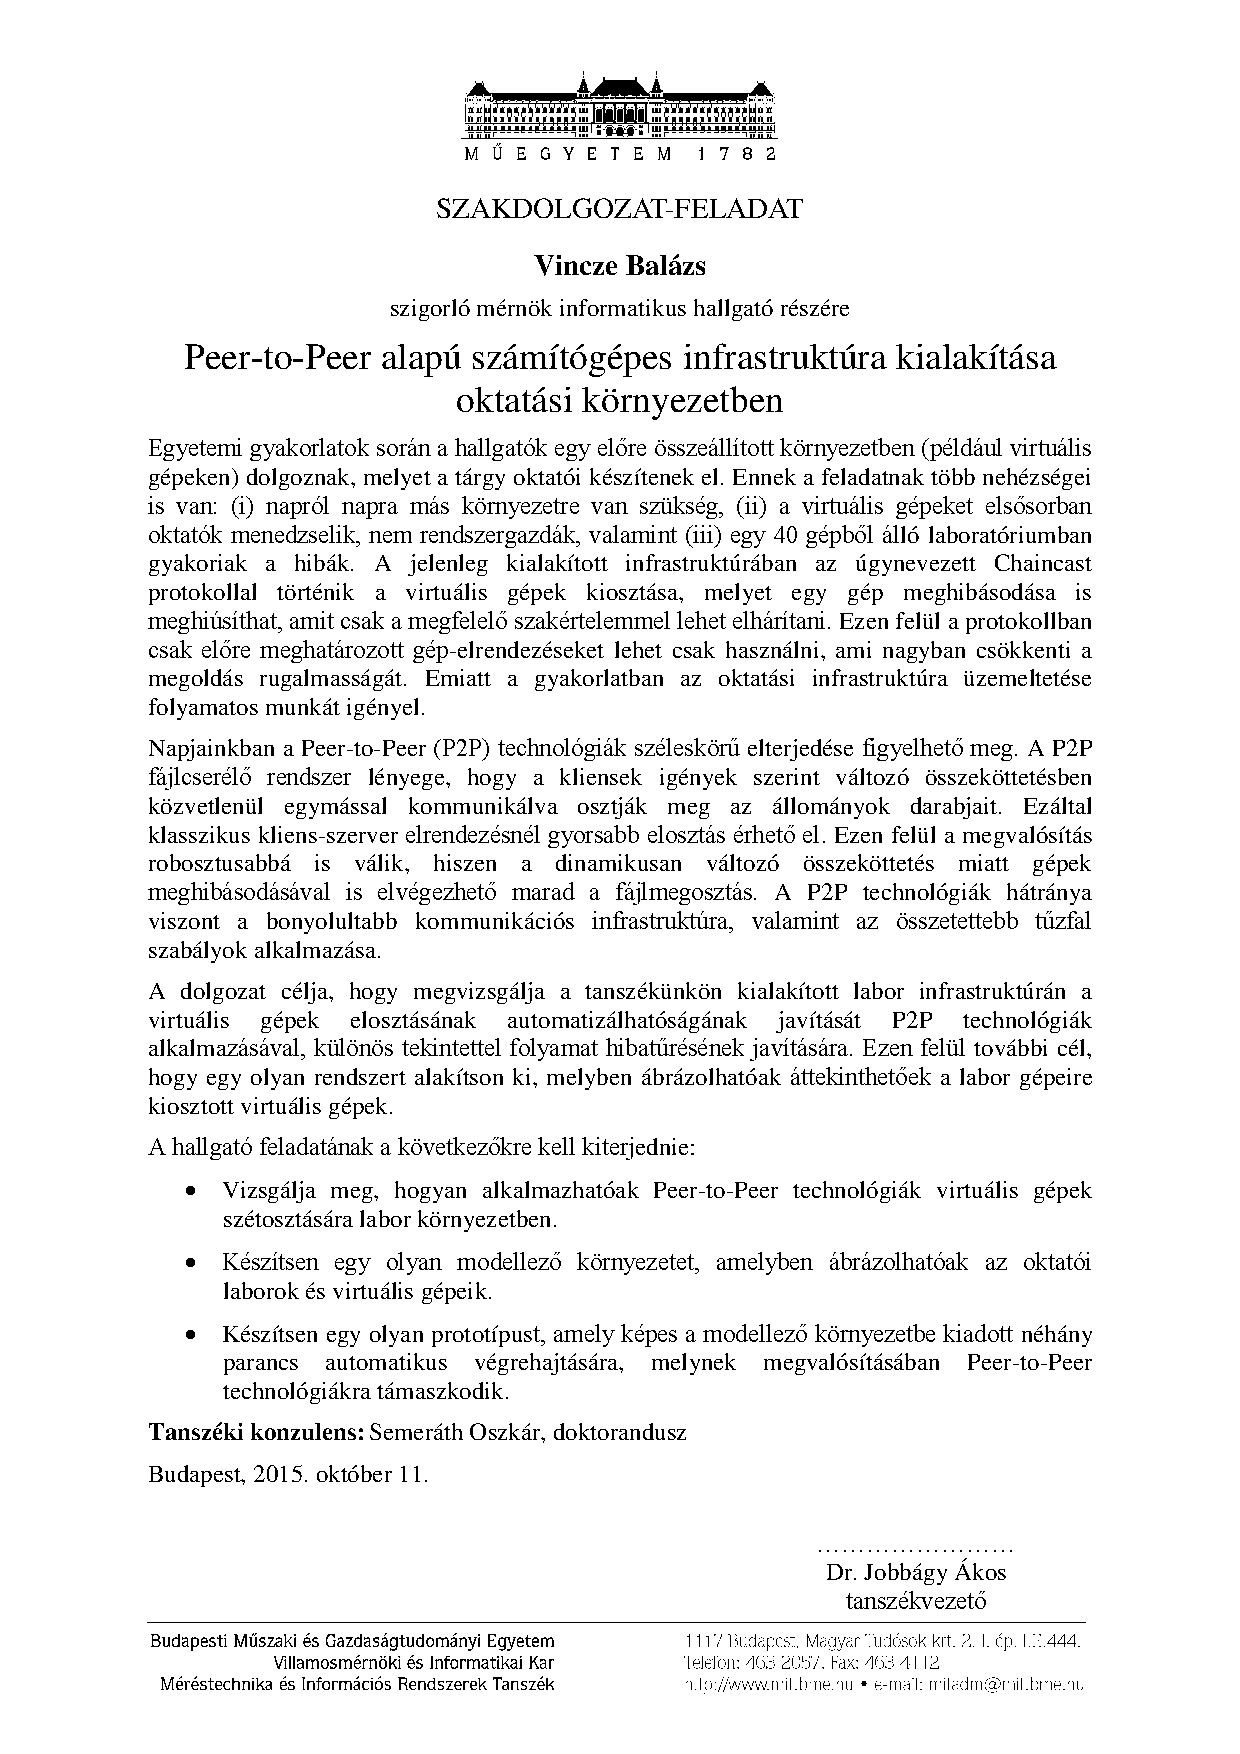
\includepdf[pages={1}]{include/taskdescr.pdf}

% The main part of the thesis
%~~~~~~~~~~~~~~~~~~~~~~~~~~~~~~~~~~~~~~~~~~~~~~~~~~~~~~~~~~~~~~~~~~~~~~~~~~~~~~~~~~~~~~
\pagenumbering{arabic}

	%----------------------------------------------------------------------------
\chapter{Bevezető} 
%----------------------------------------------------------------------------

%----------------------------------------------------------------------------
\section{Témaleírás}
%----------------------------------------------------------------------------


%----------------------------------------------------------------------------
\section{Problémafelvetés}
%----------------------------------------------------------------------------


%----------------------------------------------------------------------------
\section{Célkitűzés}
%----------------------------------------------------------------------------

%----------------------------------------------------------------------------
\section{Kontribúció}
%----------------------------------------------------------------------------

%----------------------------------------------------------------------------
\section{Hozzáadott érték}
%----------------------------------------------------------------------------

%----------------------------------------------------------------------------
\section{Korábbi munkák}
%----------------------------------------------------------------------------

%----------------------------------------------------------------------------
\section{Dolgozat felépítése}
%----------------------------------------------------------------------------


	%----------------------------------------------------------------------------
\chapter{Háttérismeretek}
\label{chp:background}
%----------------------------------------------------------------------------
Ebben a fejezetben a feladat megértéséhez szükséges technológiákat mutatom be röviden.

%----------------------------------------------------------------------------
\section{Virtuális gépek}
%----------------------------------------------------------------------------
Érdemes pár szót ejteni a virtuális gépekről, hiszen ezek terítése a programunk célja. Virtuális gépet használva egy számítógépes környezetet szimulálhatunk létrehozva egy ``teljes számítógépet egy másik számítógépen belül''. A virtualizációs megoldások közül a rendszervirtualizációs megoldásokra fókuszálunk, ahol egy egész rendszert emulálhatunk, ezen belül is az olyan megoldások, amik alkalmazásként futnak az operációs rendszerünk felett. Virtuális  gépek használatának rengeteg célja lehet. A mi esetünkben ez egységes oktatási környezet kialakítása mindegyik laborban tartott órához. Így például egy Java fejlesztéssel kapcsolatos tanórához olyan VM-et használunk, ami előre beállított fejlesztői környezetet tartalmaz.
Virtuális gépek futtatására használt programok közül talán a két legismertebb a VMWare Workstation\cite{vmware} és az Oracle VM Virtualbox\cite{virtualbox}. Ilyen gépek létrehozása alapvetően hosszadalmas folyamat, melynek lépései a következőek:

\begin{enumerate}
  \item Megadjuk a létrehozandó VM paramétereit: milyen OS-t szeretnénk rá telepíteni, mennyi erőforrást(például processzorok száma, RAM mennyisé) bocsájtunk a rendelkezésére.
  \item	Csatoljuk a telepítendő OS lemezképfájlját és elvégezzük a telepítését.
  \item A kész gépet konfiguráljuk.
  \item Feltelepítjük a szükséges alkalmazásokat.
\end{enumerate}

Ezt a folyamatot tudjuk gyorsítani és leegyszerűsíteni a Vagrant\cite{vagrant} nevű alkalmazás használatával, ami virtuális gépeket tartalmazó munkakörnyezetek kialakítására és használatára ad lehetőséget. Két legfontosabb funkciója a VM-ek automatikus létrehozása és beállítása a felhasználó által kitöltött Vagrantfile alapján, illetve ezeknek a gépeknek a futtatásának a menedzselése. A Vagrantfile tartalmazza a virtuális gép létrehozásához szükséges legfontosabb információkat: azokat a beállításokat és parancsokat, amiket egy úgynevezett ``box''-on futtatva a várt virtuális gépet eredményezi. A box az egy előre elkészített VM, amit kiindulási alapnak használhatunk. A Vagrant-ot fejlesztő cég adatbázisából\cite{atlas} szerezhetőek be a box-ok, vagy természetesen saját magunk is készíthetünk. \Aref{fig:vagrantfile}-es ábrán egy részletet láthatunk az alkalmazásunkhoz tartozó tesztkörnyezet létrehozásához szükséges Vagrantfile-ból, a fontosabb beállítások az ábrán a következők:

\begin{enumerate}
  \item \textbf{config.vm.box} -- A kiindulási box beaállítása, a ``precise'' az Ubuntu 12.04.5 LTS (Precise Pangolin)\cite{ubuntu} verzióját takarja.
  \item	\textbf{config.vm.provision} -- Ez határozza meg, hogy a virtuális gép létrehozása után azon milyen parancsokat futtasson le. A clean\_vm.sh pár mappát ürít ki a VM-en, ennek azért lehet értelme, mert beállítottuk, hogy minden indításkor fusson le ez a szkript a ``run: 'always' ''-el. Ez egy globális beállítás, mivel ``config.''-al kezdődik, így minden ezzel a Vagrantfile-al létrehozott VM-re vonatkozni fog.
  \item \textbf{config.vm.define} -- Ezzel a paranccsal definiálhatunk egy létrehozandó VM-et.
  \item \textbf{seed.vm.hostname} \& \textbf{seed.vm.network} - Virtuális gép neve és hálózati beállításai.
  \item \textbf{seed.vm.provision} -- Ugyanaz, mint a config.vm.provision, viszont kizárólag erre a VM-re vonatkozik, itt adjuk meg a seed nevű gép telepítőszkriptjét.
\end{enumerate}
 
Megfigyelhettük, hogy lehetőségünk van tetszőleges szkript futtatására a virtuális gép készítése közben, így gyakorlatilag tetszőleges VM létrehozására használható a Vagrant.

\begin{figure}[ht]
	\centering
	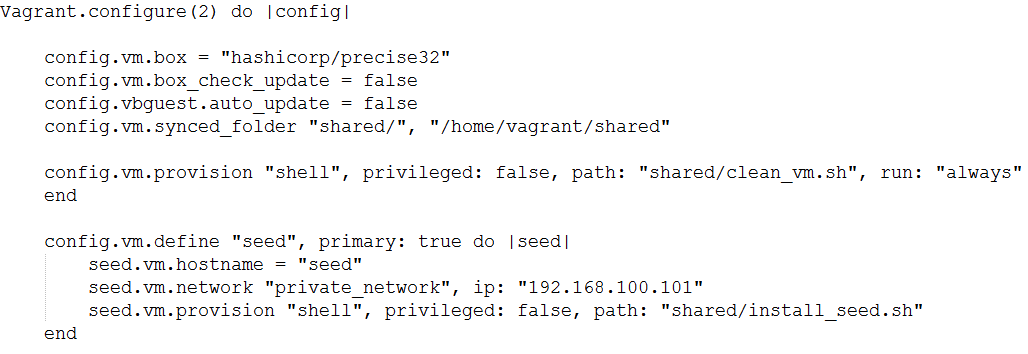
\includegraphics[width=140mm, keepaspectratio]{figures/vagrantfile.png}
	\caption{Egy Vagrantfile tartalma (részlet)}
	\label{fig:vagrantfile}
\end{figure}

\Aref{fig:vmcreate}-es ábra egy virtuális gép létrehozásának folyamatát ábrázolja mind a Vagrant által létrehozott, mind a mi általunk manuálisan készített VM esetére.

\begin{figure}[ht]
	\centering
	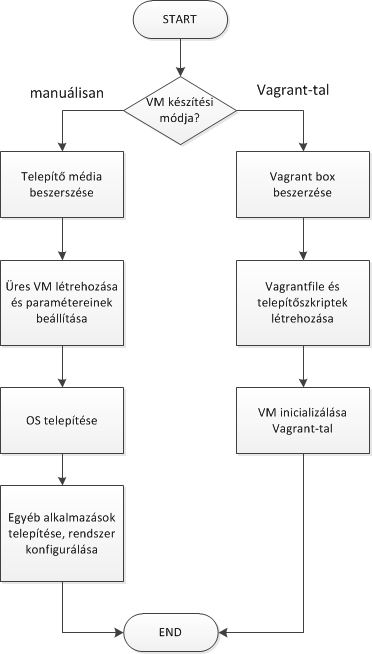
\includegraphics[height=140mm, keepaspectratio]{figures/vmcreate.png}
	\caption{Virtuális gép létrehozásának a folyamata}
	\label{fig:vmcreate}
\end{figure}

Egy virtuális gép reprezentálásához a gazdagépen alapvetően háromféle fájl szükséges legalább:

\begin{itemize}
	\item Egyik a futtatásához szükséges konfigurációs beállításokat írja le (VM metaadatai, szükséges erőforrások stb.).
	\item Másik a VM által használt virtuális lemezeken található adatokat tartalmazza.
	\item Opcionálisan lehetnek úgynevezett snapshot-ok is, amelyek egy konkrét állapotát írják a virtuális gépnek, ahova bármikor visszaállítható.
\end{itemize}

Ezeket a fájlokat terítjük a laborban.
%----------------------------------------------------------------------------
\section{Peer-to-peer fájlátvitel} 
\label{sect:p2p}
%----------------------------------------------------------------------------
A Peer-to-Peer(P2P) hálózat olyan, aminek a csomópontjai nem egy kitüntetett géppel 
kommunikálnak, hanem közvetlenül egymással. A klasszikus kliens-szerver és a P2P hálózat felépítését
\aref{fig:networkcomparison}-as ábra szemlélteti.

\begin{figure}[ht]
	\centering
	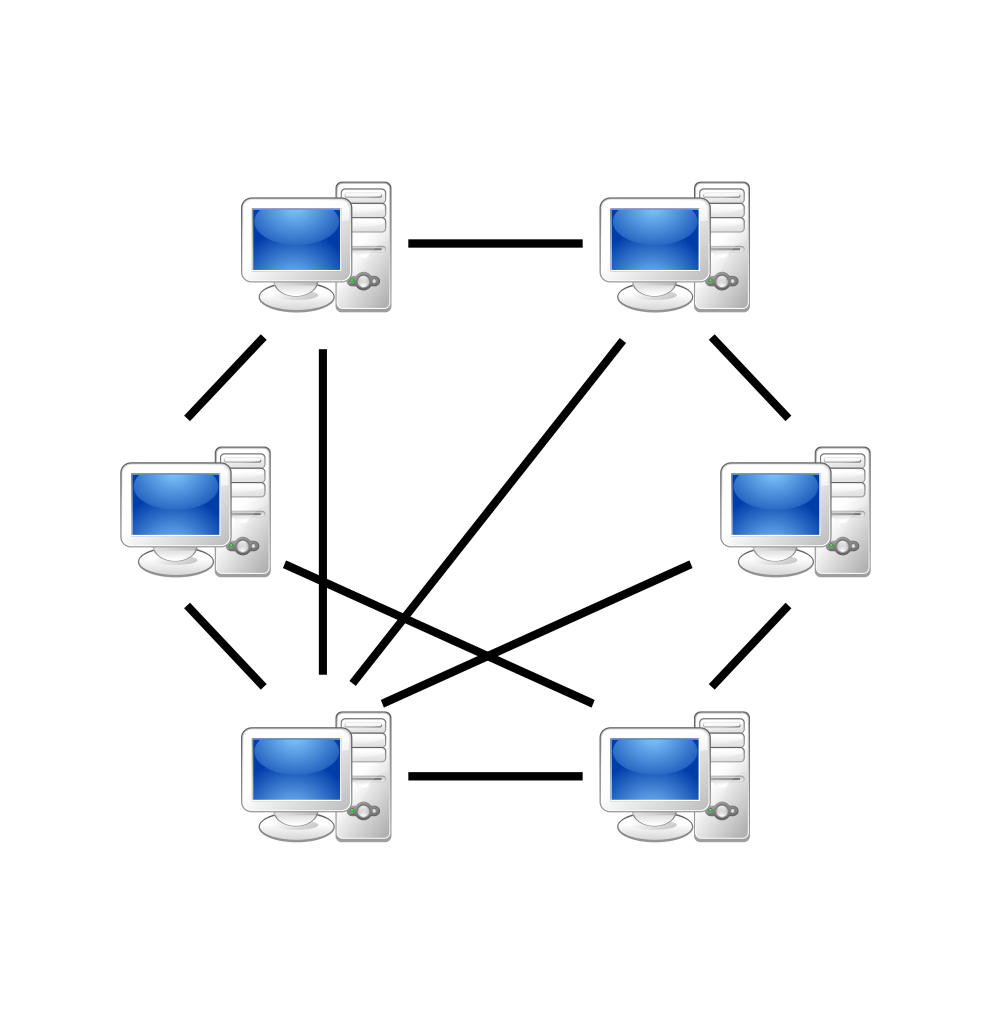
\includegraphics[width=50mm, keepaspectratio]{figures/P2P-network.png}\hspace{1cm}
	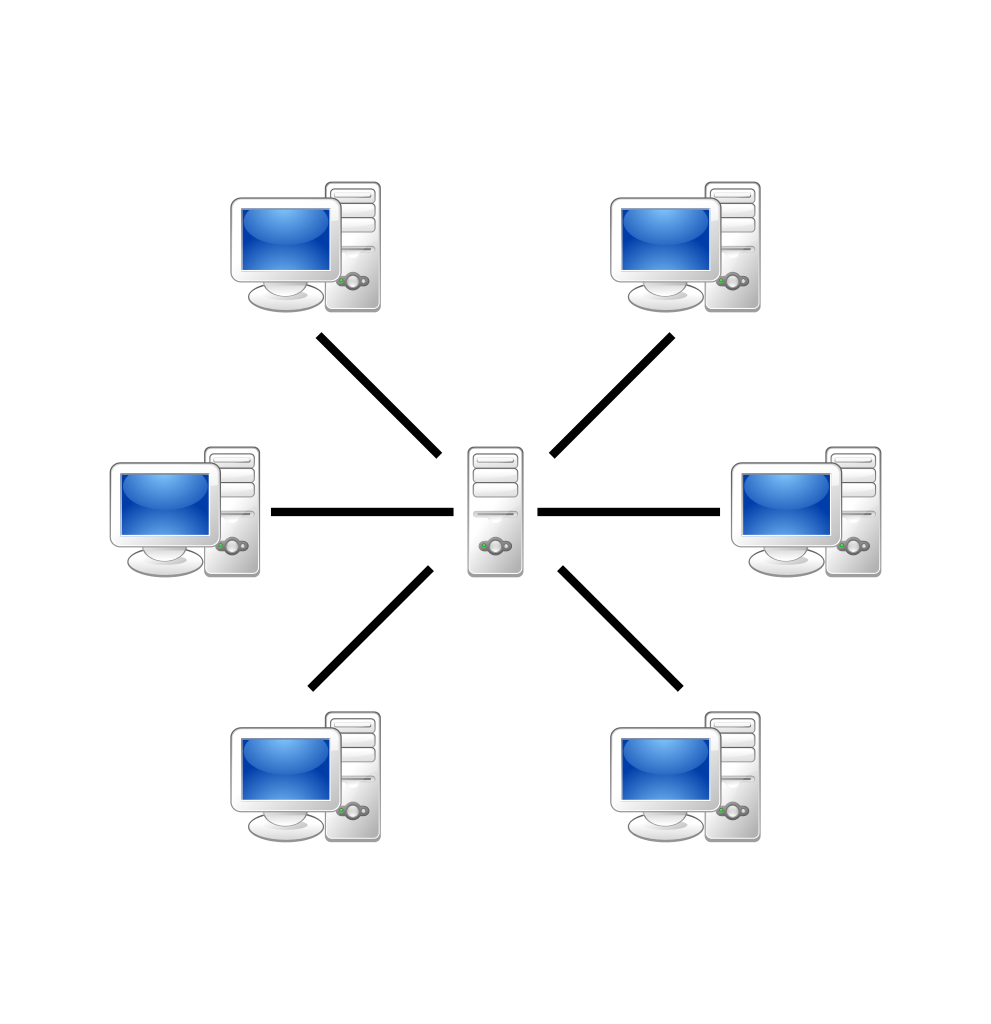
\includegraphics[width=50mm, keepaspectratio]{figures/Server-based-network.png}
	\caption{P2P és kliens-szerver alapú hálózat. \\(\textit{forrás: https://en.wikipedia.org/wiki/Peer-to-peer})}
	\label{fig:networkcomparison}
\end{figure}

P2P hálózat használatának fő előnye a robusztusság és a skálázhatóság, mivel nincs központi elem,
aminek a meghibásodása szolgáltatáskiesést okozhatna, illetve a hálózat min (például P2P alapú fájlmegosztás esetén a letöltés mellett fel is tölt). Hátrányai közül a két legjelentősebb a nehezebb karbantarthatóság és az internetszolgáltató-oldali forgalomkorlátozások miatt fellépő sebességproblémák.

A P2P alapú technológiák egyik legnagyobb felhasználási területe a tartalomszolgáltatás, ezen belül
az egyik legismertebb ilyen technológiát használó protokoll a Bittorrent. A Bittorrent~\cite{cohen2008bittorrent} protokollt
fájlmegosztásra használjuk, a mögötte álló alapvető ötlet az, hogy a megosztandó fájlokat
feldaraboljuk, és a letöltőknek ezeket a darabokat nem ugyanolyan sorrendben adjuk oda, így ők a
hiányzó darabokat egymástól is tudják tölteni. Ahhoz, hogy a letöltők megtalálják egymást, illetve a kész fájlt feltöltőket, az ún. \textbf{tracker} segít, ami adott átvitel résztvevőinek (a ``\textbf{swarm}'') adatainak tárolásáért felel. A Bittorrent terminológiájában a teljes fájlal rendelkező, már csak feltöltést végzőket \textbf{seed}-nek, a letöltőket, akik persze fel is töltenek \textbf{leecher}-nek vagy peer-nek nevezik. A tracker kiesése esetén léteznek más módszerek is a többi swarm-tag megtalálására, többek között a DHT\cite{rescorla2006introduction}(distributed hash table - elosztott hashtábla) használata, viszont esetünkben ez nem opció, mert az egyetem szabályzata tiltja a Bittorrent protokoll használatát (legalábbis a ``nagyvilág'' felé), a DHT bekapcsolása esetén pedig nem tudjuk a laborgépeinken futó torrentkliensek közti forgalmat a helyi hálóra izolálni.

Látszik, hogy torrent alapú fájlátvitel megvalósításához legkevesebb ezekre lesz szükségünk:
\begin{itemize}
	\item Minden laborgépen egy torrentkliensre
	\item Saját torrent tracker-re
	\item Seed gép kijelölésére
	\item Egy olyan programra, ami ezek működését vezérli
\end{itemize}
Az itt felsorolt elemekből felépülő terítési megoldás leírásához lásd majd \aref{design_apparchi}-as fejezetet. 

Gépeinkre telepítendő torrentkliens esetében az rtorrent-re\cite{sundell2012libtorrent} esett a választás, mivel szükségünk van arra, hogy olyan klienst használjunk, amit a háttérben is tudunk futtatni, illetve az állapota valami módon távolról is lekérhető legyen. Az rtorrent rendelkezik egy XMLRPC\cite{merrick2006xml} alapú interfésszel, aminek segítségével távolról is vezérelhetővé válik. Ilyen interfészt használ a számos rtorrent-hez írt webes felület is, például a legismertebb ruTorrent\cite{rutorrent}. Természetesen minden rtorrent-et futtató gépre telepítenünk kell egy webszervert is, ami az XMLRPC kéréseinket eljuttatja magának a torrentkliensnek, itt a választás az apache-ra\cite{fielding1997apache} esett főleg könnyű telepítése és konfigurálása miatt.

Tracker-ből az opentracker nevű került fel egy gépre (az egyszerűség kedvéért arra, amelyiket a terítések során seed-nek fogunk használni). Választásunk rá azért esett, mert különösebb funkcionális különbség nincs a lehetséges jelöltek között, ezt viszont könnyen lehet telepíteni a laborgépeken futó operációs rendszer csomagkezelőjéből. Amiről még eddig nem esett szó, az a protokoll működéséhez szükséges, metaadatokat tartalmazó fájl, a torrentfájl. Ez tárolja az adott letöltéshez tartozó fájlok hash-eit, amik adott fájl tartalmából előállított egyedi hexadecimális számok, tulajdonságuk, hogy ugyanarra a fájlra mindig ugyanaz a szám áll elő, másikra pedig szinte biztosan különböző, ezek alapján tudjuk ellenőrizni a letöltött adatok hibamentességét. A torrent fájl tartalmazza még ezen kívül a küldendő fájlok mappastruktúráját, metaadatait (pl. fájlnév, fájlméret) és a tracker címét. A torrentkliens és a tracker egy torrentfájlra az infohash alapján hivatkozik, ami a torrentfájl hash-ének kódolásával kapható meg, erre nekünk később akkor lesz szükségünk, amikor majd a terítés közben annak állapotának lekérésekor hivatkozni akarunk egy átvitelre.

Torrentfájlok létrehozására az mktorrent-et\cite{mktorrent} fogjuk használni.

\Aref{fig:torrentflow}-es ábrán egy fájl torrent alapú terítésének a folyamatát illusztrálja, onnan kezdve, hogy a fájl már a seed gépre van másolva odáig, hogy elkezdődik a célgépek által a fájl letöltése.

\vspace{0.5cm}

\begin{figure}[ht]
	\centering
	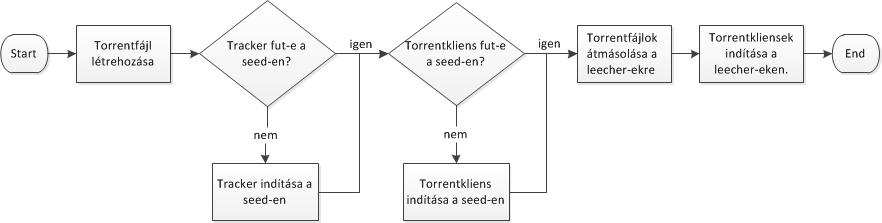
\includegraphics[width=150mm, keepaspectratio]{figures/torrentflow.png}
	\caption{Egy fájl torrent alapú terítésének folyamata.}
	\label{fig:torrentflow}
\end{figure}


%----------------------------------------------------------------------------
\section{Metamodellezés}
%----------------------------------------------------------------------------
Egy fájlterítés indításához két dologra van szükségünk, hogy mit és hova szeretnénk teríteni. Előző kérdésre \aref{sect:p2p}-es fejezet választ adott, az utóbbira ez fog. A ``hovának'' megadását sokféleképpen elképzelhetjük,  felhasználói szemszögből az lenne a legjobb, ha egyszerűen azt mondhatnánk, hogy ``az IB413-as laborban a Mérés Labor 4. tárgyhoz tartozó környezet terüljön.'' Fontos, hogy képes legyen az alkalmazás egy ilyen kérést végrehajtani, ha a kérést számára értelmezhetőbb formában adjuk át. 
A virtuális gép terítési feladatokat érdemes egy saját, úgynevezett szakterület-specifikus nyelven modellezni (angolul Domain-Specific Language, DSE). Egy szakterület-specifikus nyelv legfőbb koncepcióit, kapcsolatait és alapvető struktúráját határozza meg a metamodell. Például egy labor metamodellje alatt egy olyan nyelvet kell elképzelni, amiben leírható tetszőleges oktatási labor. \Aref{fig:emfobj}-ös ábra egy ilyen metamodell egyik osztályát ábrázolja.

\vspace{0.5cm}

\begin{figure}[ht]
	\centering
	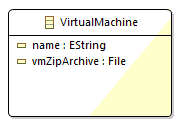
\includegraphics[width=50mm, keepaspectratio]{figures/binf_emf_1.png}
	\caption{Metamodell osztály - \textit{Terítendő virtuális gépeket ábrázolja, lehetséges attribútumai a VM neve és a hozzá tartozó fájlokat tároló tömörített állomány elérési útvonala.}}
	\label{fig:emfobj}
\end{figure}

Metamodell osztályok között lehetnek kapcsolatok is, amelyek közül a két legfontosabb a tartalmazás(kompozíció) és a referencia. \Aref{fig:emfcomp}-os ábrán egy kompozícióra, \ref{fig:emfref}-esen egy referenciára láthatunk példát.

\vspace{0.5cm}

\begin{figure}[ht!]
	\centering
	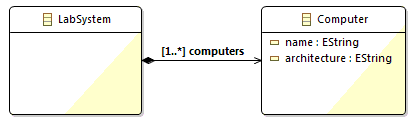
\includegraphics[width=115mm, keepaspectratio]{figures/binf_emf_2.png}
	\caption{Kompozíció - \textit{Azt írja le, hogy a laborunk tetszőleges számú (minimum 1 darab) számítógépből áll.}}
	\label{fig:emfcomp}
\end{figure}

\vspace{0.5cm}

\begin{figure}[ht!]
	\centering
	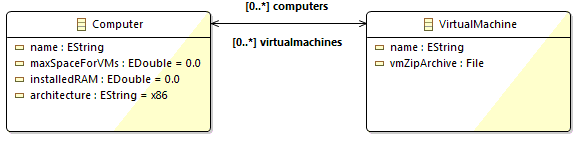
\includegraphics[width=150mm, keepaspectratio]{figures/binf_emf_3.png}
	\caption{Referencia - \textit{Egy számítógépen tetszőleges VM lehet, illetve egy VM tetszőleges számú számítógépen lehet rajta.}}
	\label{fig:emfref}
\end{figure}


Egy ilyen metamodell segítségével létrehozhatunk egy, a laborok leírására alkalmas modellezési nyelvet, ennek a gyakorlati használatát segíti az Eclipse Modeling Framework\cite{steinberg2008emf}. Az EMF-el az elkészített metamodell használatát tudjuk Java programokba integrálni, továbbá szerkesztőfelületet is létre tud hozni adott modell adatainak kitöltéséhez. Az EMF által, a metamodellből generált forráskódot használva a programunk egyszerűen be tud tölteni modellfájlokat, így tehát a terítést tudjuk vezérelni az EMF-ben létrehozott modellel, ami leírja a labor felépítését és a terítés célállapotát.
	%----------------------------------------------------------------------------
\chapter{Tervezés}
\label{chp:design}
%----------------------------------------------------------------------------
Ebben a fejezetben 



\section{A labor modelljének tervezése}
\label{design_model}

\Aref{fig:designmodelparts}-es ábra mutatja meg, hogy milyen 3 részere vághatjuk a terítéshez szükséges modellt.

\begin{figure}[ht]
	\centering
	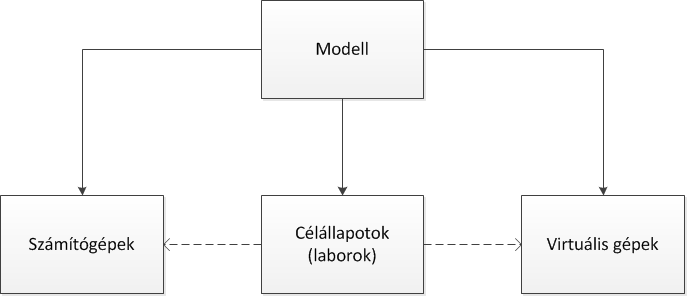
\includegraphics[width=100mm, keepaspectratio]{figures/design_modelparts.png}
	\caption{}
	\label{fig:designmodelparts}
\end{figure}

\Aref{fig:designcomputers}-s ábrán a számítógépeket tartalmazó darab részletesebb leírása van.

\begin{figure}[ht]
	\centering
	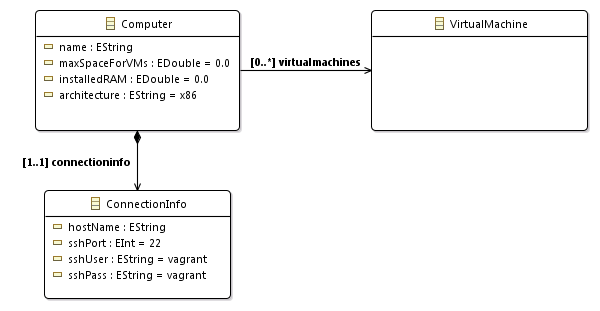
\includegraphics[width=110mm, keepaspectratio]{figures/design_computer.png}
	\caption{}
	\label{fig:designcomputers}
\end{figure}

\Aref{fig:designvm}-s ábrán a virtuális gépeket tartalmazó darab részletesebb leírása van.

\begin{figure}[ht]
	\centering
	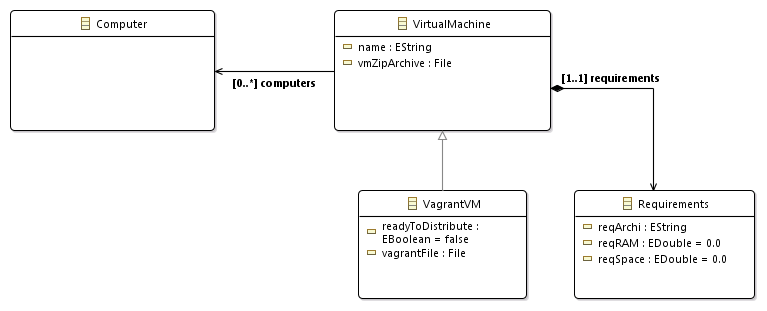
\includegraphics[width=130mm, keepaspectratio]{figures/design_vm.png}
	\caption{}
	\label{fig:designvm}
\end{figure}

\Aref{fig:designlab}-s ábrán a terítés végállapotát (pc->vm összerendelések) tartalmazó darab részletesebb leírása van.

\begin{figure}[h!]
	\centering
	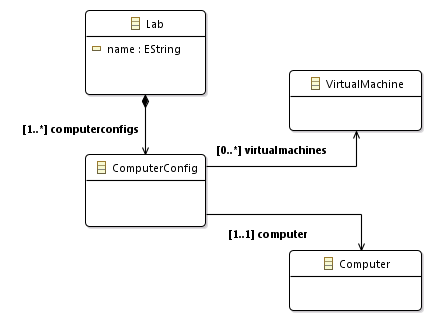
\includegraphics[width=100mm, keepaspectratio]{figures/design_lab.png}
	\caption{}
	\label{fig:designlab}
\end{figure}

\section{Terítési műveletek a modellen}

Annak a megtervezésére, hogy egy fájlterítési folyamat hogyan zajlik érdemes azt kisebb darabokba vágni, azt definiálni egyszerű műveletekkel.
Az előbbi fejezetben ismertetett modellre definiálok itt terítési műveleteket, és megkísérlem leírni segítségükkel az egész fájlterítési folyamatot.
Az egyszerű műveleteket a következő formátumban fogom definiálni: MŰVELET\_NEVE(paraméter1\_neve: paraméter1\_típusa, paraméter2\_neve\ldots).

A modellen értelmezett terítési műveletek: [a többi modellen értelmezhető művelet, amitől teljes rendszerré válik a dolog, de a terítésnél nem relevánsak kellenek-e? Gondolok itt azokra, amik üres modellt hoznak létre, hozzáadnak pc-t/vm-et/lab-et az erőforrásokhoz.]

\begin{itemize}
  \item KÜLÖNBSÉG(cél: Lab, erőforrások: LabSystem): Ez a művelet a paraméterei között különbséget képez, vagyis a Lab-ből kiszedi azokat a (Computer, VirtualMachine) párokat, amik a LabSystem-ben már szerepelnek. Ennek az a célja, hogy a terítendő VM-ek közül kiszűrje azokat, amelyek már ott vannak, ahova terítenénk őket. Visszatérési érték: Lab, ami a duplikátumokat nem tartalmazza.
  \item TÖRÖL(törlendő\_vm : VirtualMachine, melyik\_gépekről: List<Computer>): Ezzel a művelettel törölhetjük a második paraméter Computer-eket tartalmazó lista összes eleméről az adott virtuális gépet. Visszatérési érték: nincs, a paraméterként kapott gépeknek módosítja a tartalmát.
  \item KOMPATIBILIS\_E(pc: Computer, vm: VirtualMachine): Arra a kérdésre válaszol, hogy adot VM kompatibilis-e a Computer-rel. Ellenőrzi az architektúrák megfelelését, a memória és a szabad lemezterület méretét. Visszatérési érték: IGAZ vagy HAMIS.
  \item FELTÖLT(vm: VirtualMachine, pc: Computer): Feltölti a VM-et a Computer-re, vagyis hozzáadja annak a \code{virtualmachines} listájához. Visszatérési érték: nincs, amennyiben már ott található a feltöltendő VM a PC-n, akkor a művelet nem csinál semmit.
\end{itemize}

Az előbbiek segítségével már felírható a TERÍTÉS(cél: Lab, erőforrások: LabSystem) művelet: [talán ábrával és nem pszeudokóddal?]

\code{TERÍTÉS(cél: Lab, erőforrások: LabSystem):}\\
\indent \code{duplikátumok\_nélküli\_cél = KÜLÖNBSÉG(cél, LabSystem)}\\
\indent \indent \code{FOR minden ComputerConfig a duplikátumok\_nélküli\_cél-ban}\\
\indent \indent \indent	\code{FOR minden VirtualMachine a ComputerConfig.Virtualmachines-ben}\\
\indent \indent \indent	\code{HA(KOMPATIBILIS(ComputerConfig.Computer, VirtualMachine))}\\
\indent \indent \indent \indent	\code{AKKOR FELTÖLT(VirtualMachine, ComputerConfig.Computer)}


\section{Fájlterítő alkalmazás architektúrája}
\label{design_apparchi}

\Aref{fig:designoverview}-es ábra fogja elmagyarázni az új terítési megoldás alapvető működési elvét: beolvassuk a modellt, ami alapján az egyik gépet seed-nek kiválasztva megcsináljuk a torrentes terítés. Az alkalmazás a terítésben szereplő gépektől (a torrent swarm-ja) futás közben a terítés állapotáról kér le információkat.

\begin{figure}[ht]
	\centering
	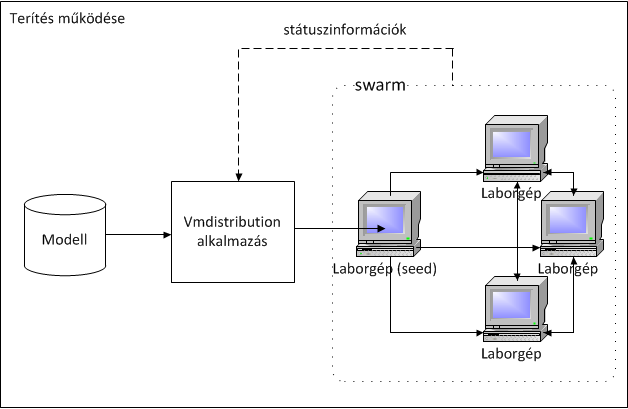
\includegraphics[width=130mm, keepaspectratio]{figures/design_overview.png}
	\caption{}
	\label{fig:designoverview}
\end{figure}

\Aref{fig:designprotocols}-es ábrán látjuk, hogy a terítés egyes szereplői hogyan és milyen protokollokat használva kommunikálnak egymással. [kell-e vajon ehhez, ill. az előzőhöz a tárhely, ahol a virtuális gépeket tároljuk?]

\begin{figure}[ht]
	\centering
	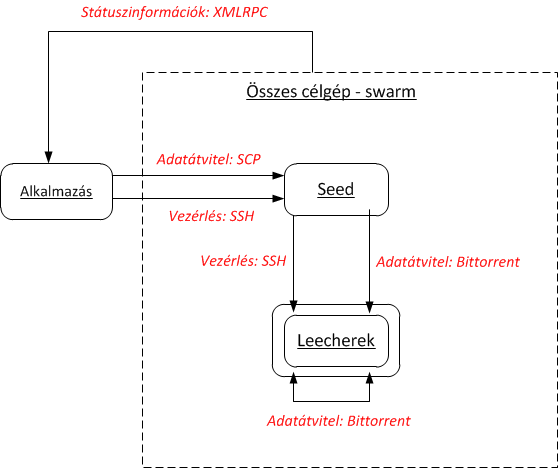
\includegraphics[width=140mm, keepaspectratio]{figures/design_protocols.png}
	\caption{.}
	\label{fig:designprotocols}
\end{figure}


	%----------------------------------------------------------------------------
\chapter{Implementáció}
\label{chp:implementation}
%----------------------------------------------------------------------------
Ebben a fejezetben a fájlterítő alkalmazás implementációjának részleteit mutatom be, mint annak követelményeit, konfigurálását, használatát, illetve felépítését.
Az alkalmazást Vmdistribution-nek neveztem el, forráskódja elérhető GitHub-on a cvswarrior/vmdistribution repository alatt\cite{vmdistribution}.

%----------------------------------------------------------------------------
\section{Követelmények és konfiguráció}
%----------------------------------------------------------------------------

A \textit{\textbf{Vmdistribution-t futtató}} gépen telepítve kell lennie a következőknek:
\begin{itemize}
  \item Egy JVM-nek\cite{stark2001java}, ami támogatja az 1.7-es verziójú Java-t(például az aktuális legfrissebb JRE az Oracle-től\cite{oraclejre}.).
  \item Vagrant 1.7.4, vagy frissebb
  \item Virtuális gépek kezelésére alkalmas szoftver - bármelyik Vagrant által támogatott\cite{vagrantproviders} (javasolt VirtualBox vagy VMWare Workstation használata)
\end{itemize}
Értelemszerűen azért van szükségünk JVM-re, hogy Java nyelven íródott alkalmazásokat tudjunk futtatni, Vagrantra és mondjuk VirtualBoxra pedig azért, hogy lehetőség legyen Vagrant által létrehozandó VM-ek terítésére.

A \textit{\textbf{labor}} gépeire vonatkozó követelmények:
\begin{itemize}
  \item Debian-alapú Linux disztribúció (természetesen a függőségeket manuálisan fordítva tetszőleges disztribúció használható)
  \item SSH szerver engedélyezett jelszó alapú bejelentkezéssel
\end{itemize}
Az SSH szerverre azért van szükség, hogy tudjunk az összes laborgéppel kommunikálni, azokat távolról vezérelni, Debian-alapú disztribúcióra pedig, mert annak a csomagkezelezője segítségével van az alkalmazásunk függőségeinek nagy része telepítve.

A \textit{\textbf{labor}} gépeire a mellékelt telepítőszkriptek futtatásával, vagy manuálisan a következő alkalmazásokat kell telepíteni:
\begin{itemize}
  \item tmux
  \item rtorrent 0.9.6 vagy frissebb
  \item	sshpass\footnote{Csak azokon a gépeken szükséges, amiket terítéskor seed-nek akarunk használni}
  \item opentracker\footnotemark[1]
  \item mktorrent\footnotemark[1]
  \item apache (vagy egyéb XMLRPC protokollt kezelni tudó webszerver)
\end{itemize}
Az rtorrent tölti be a torrentkliens szerepét, az opentracker a tracker-ét, az apache segítségével tudja a gép a beérkező XMLRPC hívásokat fogadni és az rtorrent-nek továbbítani. Tmux segítségével tudunk távolról, szkriptből indított programot a ``háttérben'' futtatni, jelen esetben az rtorrent-et és az opentracker-t. Az sshpass lehetővé teszi, hogy a seed gép jelszavas bejelentkezést használva automatizáltan tudjon SSH kapcsolatot létesíteni a többi laborgéppel. Torrent fájlokat az mktorrent programmal fogunk létrehozni a seed-en.

%----------------------------------------------------------------------------
\section{Használat}
%----------------------------------------------------------------------------

Az alkalmazás használatához először is szükségünk van a labor modelljét leíró fájlra, ami tartalmazza annak felépítését és a lehetséges célállapotokat. Ezt legegyszerűbben az EMF által generált szerkesztővel lehet létrehozni. A program egy parancssori Java alkalmazás, ezért onnan a következőképpen indíthatjuk el:

\code{java -jar vmdistribution.jar modelfile goal\_lab logging\_level}

A 'modelfile' helyére értelemszerűen a modellt tartalmazó fájl elérési útvonala, a ``goal\_lab''-hoz a célállapotnak a neve, a ``logging\_level''-hez pedig a naplózási szint kerül. A naplózási szint alatt azt kell érteni, hogy mennyire részletes lesz a program futásának a kimenete, a lehetséges értékek részletesség szerinti növekvő sorrendben: WARNING, INFO, FINE, FINER.
A fájlterítés futását a STOP vagy S parancsokkal lehet megszakítani. Amennyiben véget ért a terítés a modellfájlban frissülni fognak a megfelelő Computer és VirtualMachine objektumok a terítés eredménye alapján.

%----------------------------------------------------------------------------
\section{Az alkalmazás felépítése}
%----------------------------------------------------------------------------
\label{impl_app}

\Aref{fig:packagediag}-es ábrán az alkalmazást felépítő fontosabb Java osztályokat láthatjuk a csomagjaik szerint, azok egymástól való függéseit jelölve. Az ábra után következő táblázat tartalmazza a felrajzolt osztályok rövid leírását.

\begin{figure}[ht]
\centering
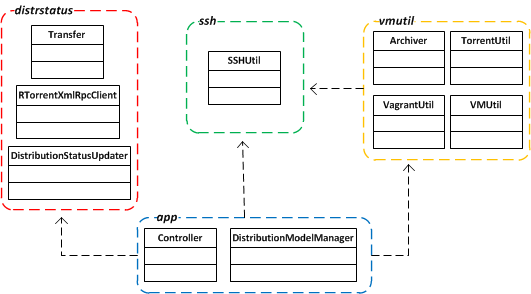
\includegraphics[width=150mm, keepaspectratio]{figures/packagediag.png}
\caption{Vmdistribution osztályai és package-ei}
\label{fig:packagediag}
\end{figure}

\definecolor{orange}{RGB}{255,127,0}
\definecolor{lightred}{RGB}{255,99,71}
\definecolor{seagreen}{RGB}{46,139,87}
\definecolor{skyblue}{RGB}{135,206,250}

\begin{center}
	\begin{tabular}{|>{\centering\arraybackslash}m{45mm}|>{\centering\arraybackslash}m{95mm}|}
		\hline
		\textbf{Osztály neve}&\textbf{Funkciójának rövid leírása}\\
		\hline
		\cellcolor{skyblue}UseModel & \cellcolor{skyblue}Az alkalmazás fő osztálya, ez tartalmazza main függvényt és vezérli a terítési folyamatot.\\ 
		\hline
		\cellcolor{skyblue}EMFModelUtil & \cellcolor{skyblue}A labor modelljét kezeli: betölti, futtatás után elmenti, illetve műveleteket tud végezni rajta (pl. kezdeti és végállapot közti különbség meghatározása\\
		\hline
		\cellcolor{seagreen}SSHUtil & \cellcolor{seagreen}SSH kapcsolatot tud létrehozni és azon keresztül távoli gépekre parancsokat küldeni és SCP protokollt használva fájlokat küldeni.\\
		\hline
		\cellcolor{orange}VMUtil & \cellcolor{orange} Virtuális gépek seed-re történő másolásáért felel\\
		\hline
		\cellcolor{orange}TorrentUtil &\cellcolor{orange}Torrentfájlok létrehozását, seed-elés leech-elés indítását vezérli a laborgépeken az SSHUtil osztályt használva. \\
		\hline
		\cellcolor{orange}VagrantUtil &\cellcolor{orange} Vagrant alapú virtuális gépek inicializálását végzi el a lokális gépen futó Vagrant segítségével.\\
		\hline
		\cellcolor{orange}Archiver &\cellcolor{orange} ZIP formátumú tömörített fájlokat hoz létre(új Vagrant-os VM-ekből).\\
		\hline
		\cellcolor{lightred}Transfer &\cellcolor{lightred} Egy VM->laborgép adatátvitelt reprezentál, tárolja a letöltés aktuális állapotát (mennyi van még hátra, sebesség stb.)\\
		\hline
		\cellcolor{lightred}RTorrentXmlRpcClient &\cellcolor{lightred} Kapcsolatot létesít XMLRPC protokollon keresztül a laborgépek torrentklienseivel.\\
		\hline
		\cellcolor{lightred}DistributionStatusUpdater &\cellcolor{lightred} Torrentkliensektől kéri le valós időben a terítés aktuális állapotát és frissíti az összes Transfer objektumot.\\
		\hline
	\end{tabular}
\end{center}

%----------------------------------------------------------------------------
\section{Egy konkrét terítés végigkövetése}
%----------------------------------------------------------------------------

Érdemes a Vmdistribution egy futását végigkövetni, így még részletesebben megismerhető a Torrent alapú terítés folyamata:
A futtatást a program fejlesztésére használt gépen végeztem el, a terítésben résztvevő gépek Vagrant-tal létrehozott, VirtualBox által futtatott virtuális gépek, amelyeken az operációs rendszer 32-bites 12.04 verziójú Ubuntu\cite{ubuntu}. A virtuális gépekre csak a legszükségesebb szoftverek lettek telepítve, egymással és a gazdagéppel egy közös privát hálózaton voltak. A program futtatásához megadott labormodell fontosabb paraméterei:

\begin{itemize}
  \item Két különböző virtuális gép van benne: egy mi általunk és egy Vagrant által készített
  \item 6 darab számítógép, amik közül az egyik dedikált seed (labpc101-105, seed nevűek)
  \item Olyan célállapot, amivel minden lehetséges hiba meg fog jelenni a futás során
\end{itemize}

Mielőtt végigkövetnénk a futtatást érdemes végiggondolni, hogy mi lenne az elvárt eredmény, milyen fontosabb lépéseket és milyen sorrendben fog a program végrehajtani:

\begin{enumerate}
  \item Figyelmeztetés, hogy 105 és 104-re semelyik, 103 és 102-re pedig egyik virtuális gép nem fog terülni bizonyos problémák miatt
  \item Vagrant-os VM inicializálása, majd becsomagolása egy zip archívumba
  \item Mindkét VM felmásolása a seed gépre, mindkettőhöz torrent fájl létrehozása
  \item Torrentkliens futtatása a seed gépen
  \item Torrent fájlok átmásolása a labpc101-103 gépekre
  \item Torrentkliens futtatása a labpc101-103 gépeken
  \item A letöltések sikeres befejezése után a modell frissítése
\end{enumerate}

A program indítása után rögtön a várt figyelmeztetések jelennek meg a konzolablakban, például:

\code{2015-12-08 00:21:48 WARNING hu.bme.mit.vmdistribution.app.EMFModelUtil isCompatible WARNING:\_Computer:labpc104 is not compatible with Virtual Machine:vagrantvm\_test, Not enough RAM!}

Majd meghívódik a Vagrant és létrehozza, valamint beállítja a hozzá tartozó VM-et. \Aref{fig:vboxcap}-es~ábrán látható, hogy a VirtualBox VM-eket tartalmazó mappájába már bele is került az új virtuális gép és meg is jelenik annak a felületén.

\begin{figure}[ht]
\centering
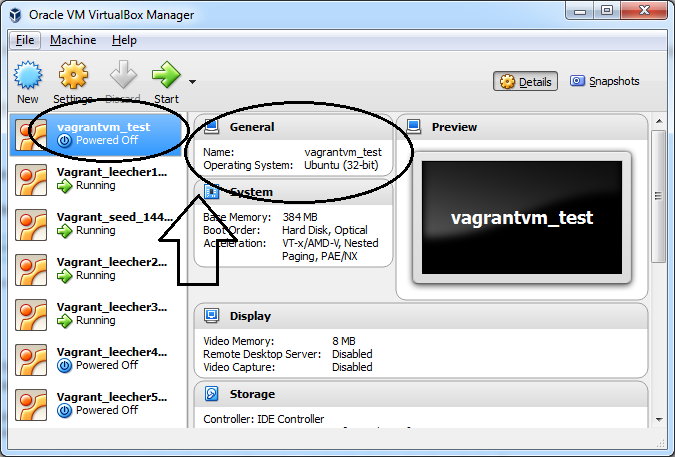
\includegraphics[width=140mm, keepaspectratio]{figures/test_vbox.png}
\caption{Vagrant által létrehozott virtuális gépek a VirtualBox-ban}
\label{fig:vboxcap}
\end{figure}
A kész virtuális gépből a program létrehoz egy tömörített .zip állományt\ldots

\code{2015-12-08 00:37:03 INFO hu.bme.mit.vmdistribution.app.vmutil.Archiver createZipArchive Creating Archive: E:\textbackslash{}vagrantvm\_test.zip}

\ldots majd a két VM felkerül a seed-re, ahogy \aref{fig:seed_files}-as~ábrán ez látszik is:  a seed-del SSH kapcsolat létesítése után kilistázzuk azoknak a mappáknak a tartalmát ahová a VM-eket tartalmazó zip fájlok, illetve az azok alapján készített torrent fájlok kerültek.

\begin{figure}[ht]
\centering
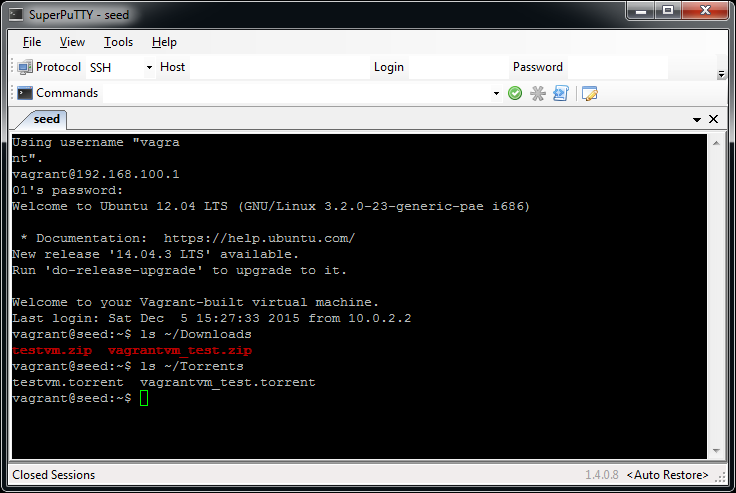
\includegraphics[width=140mm, keepaspectratio]{figures/test_seed_files.png}
\caption{Terítendő VM-ek és a torrent fájlok a seed-en}
\label{fig:seed_files}
\end{figure}

Ezután az alkalmazás a torrent fájlokat átmásolja a megfelelő célgépekre, és elindítja rajtuk a torrentklienst. A seed-en futó torrentklienst megnyitva ellenőrizhetjük, hogy elkezdődött-e az adatátvitel (\ref{fig:seed_torrent}-es ábra). A feltöltési limit kézzel alacsonyra lett állítva, hogy a folyamatok megfigyelhetőek legyenek.

\begin{figure}[ht]
\centering
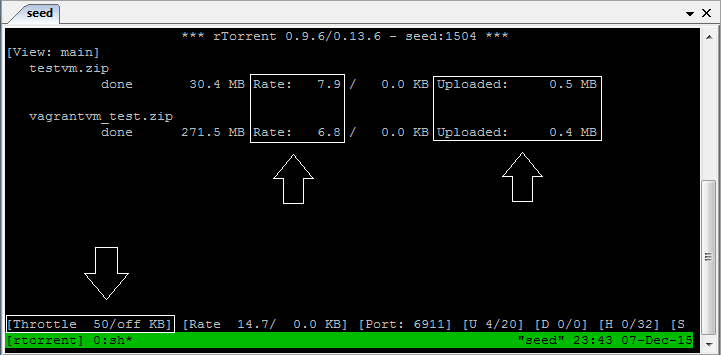
\includegraphics[width=140mm, keepaspectratio]{figures/test_seed_torrent.png}
\caption{Rtorrent: Futó feltöltések}
\label{fig:seed_torrent}
\end{figure}

A két futó fájlátvitel részleteit megnézve ellenőrizhetjük, hogy a megfelelő gépek töltenek-e le. Például a mi általunk készített VM-et tartalmazó testvm.zip-et a labpc101 és 103-nak kellene töltenie, lásd \ref{fig:seed_peers}-ös~ábra (a két gép IP címe .111 ill. .113-ra végződik).

\begin{figure}[ht]
\centering
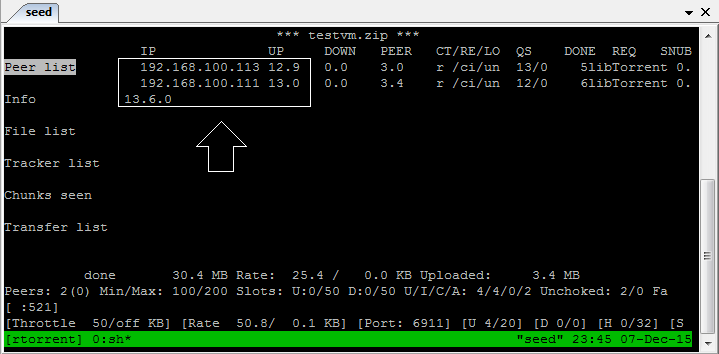
\includegraphics[width=140mm, keepaspectratio]{figures/test_seed_peers.png}
\caption{Rtorrent: Torrent részletei}
\label{fig:seed_peers}
\end{figure}

Egy pár percen belül véget is ér a terítés. A modellünket tartalmazó fájlt közelebbről megnézve ellenőrizhetjük, hogy az tényleg frissült-e, a labpc101-et reprezentáló Computer objektum például most már így néz ki:

\code{<computers virtualmachines="//@virtualmachines.1 //@virtualmachines.0" name="labpc101" maxSpaceForVMs="40000.0" installedRAM="8000.0" architecture="x64">}

A Computer-en levő virtuális gépeket a virtualmachines lista tárolja, aminek a két eleme a terített virtuális gépek objektumaira mutat.

Ez volt egy konkrét terítés folyamatának bemutatása.

	%----------------------------------------------------------------------------
\chapter{Validáció}
%----------------------------------------------------------------------------
\begin{itemize}
  \item a két alfejezet rövid tartalma jön ide
\end{itemize}

%----------------------------------------------------------------------------
\section{Tesztelés}
%----------------------------------------------------------------------------
\begin{itemize}
  \item a készített alkalmazás egy adott bemenettel történő futását kísérjük nyomon:
  \item tesztkörnyezet bemutatása, milyen szempontok alapján lett összeállítva
  \item program futásának végigkövetése (sok screenshottal)
  \item értékelés
\end{itemize}

%----------------------------------------------------------------------------
\section{Teljesítményelemzés}
%----------------------------------------------------------------------------
\begin{itemize}
  \item ide a jönnek a teljesítményelemzés eredményei, sok-sok grafikonnal:
  \item sebességösszehasonltások
  \item hibatűrési tesztek
\end{itemize}
	%----------------------------------------------------------------------------
\chapter{Összegzés}
\label{chp:summary}
%----------------------------------------------------------------------------

%----------------------------------------------------------------------------
\section{Eredmények}
%----------------------------------------------------------------------------
 
Dolgozatomban bemutattam egy modellvezérelt P2P alapú fájlterítő alkalmazás tervezését és implementációját, a következő részekre kitérve:az ezek  ismertetését sem mellőzve:

\begin{itemize}
  \item Bemutattam a megoldás megértéséhez szükséges háttérismereteket
  \item Modelleztem a megoldandó terítési feladatot, és az ahhoz használt erőforrásokat.
  \item Definiáltam a szükséges terítési műveleteket.
  \item Implementáltam a programot, illetve a hozzá kapcsolódó segédszkripteket.
  \item Teszteltem a program helyes működését.
  \item Teljesítményméréseket végeztem éles környezetben.
\end{itemize}

A feladatkiírásban felvetett összes kérdésre választ adtam, a következő helyeken:

\begin{itemize}
  \item ``Vizsgálja  meg,  hogyan  alkalmazhatóak  Peer-to-Peer  technológiák  virtuális  gépek 
szétosztására labor környezetben.'' - \ref{design_apparchi}-as fejezet
  \item ``Készítsen  egy  olyan  modellező  környezetet,  amelyben  ábrázolhatóak  az  oktatói 
laborok és virtuális gépeik.'' - \ref{design_model}-es fejezet
  \item ``Készítsen egy olyan prototípust, amely képes a modellező környezetbe kiadott  néhány
parancs  automatikus  végrehajtására,  melynek  megvalósításában  Peer-to-Peer 
technológiákra támaszkodik.'' - \ref{impl_app}-as fejezet
\end{itemize}


%----------------------------------------------------------------------------
\section{Jövőbeli munka}
%----------------------------------------------------------------------------
Az elkészített program a kitűzött feladatokat megoldja, viszont ez nem jelenti azt, hogy ne lehessen továbbfejlesztésére lehetőségeket felvetni:
\begin{itemize}
  \item Használatát felhasználóbarátabbá tenné, ha készítenénk hozzá egy grafikus felületet. Erre több lehetőség is adott: Swing\cite{zukowski2005definitive} alapú natív Java megoldás, az Eclipse fejlesztőkörnyezetbe integrálás beépülő modulként, illetve a most használt Jenkins CI rendszerből futtatás lehetőségének hozzáadása.
  \item A Vmdistribution konfigurálásának legnagyobb része a laborunk modelljének adatainak a kitöltésével jár, ezen belül is az összes számítógép releváns információinak felvitelével. Ennek az automatizálására is felkészíthetnénk a programot, vagyis arra, hogy fel tudja deríteni a környezetet, amiben fut és ez alapján inicializálja a modellt.
\end{itemize}


% Acknowledgements
%~~~~~~~~~~~~~~~~~~~~~~~~~~~~~~~~~~~~~~~~~~~~~~~~~~~~~~~~~~~~~~~~~~~~~~~~~~~~~~~~~~~~~~
%%----------------------------------------------------------------------------
\chapter*{\koszonetnyilvanitas}\addcontentsline{toc}{chapter}{\koszonetnyilvanitas}
%----------------------------------------------------------------------------

Ez nem kötelező, akár törölhető is. Ha a szerző szükségét érzi, itt lehet köszönetet nyilvánítani azoknak, akik hozzájárultak munkájukkal ahhoz, hogy a hallgató a szakdolgozatban vagy diplomamunkában leírt feladatokat sikeresen elvégezze. A konzulensnek való köszönetnyilvánítás sem kötelező, a konzulensnek hivatalosan is dolga, hogy a hallgatót konzultálja.

% List of Figures, Tables - not needed
%~~~~~~~~~~~~~~~~~~~~~~~~~~~~~~~~~~~~~~~~~~~~~~~~~~~~~~~~~~~~~~~~~~~~~~~~~~~~~~~~~~~~~~
%	\listoffigures\addcontentsline{toc}{chapter}{\abrakjegyzeke}
%	\listoftables\addcontentsline{toc}{chapter}{\tablazatokjegyzeke}

% Bibliography
%~~~~~~~~~~~~~~~~~~~~~~~~~~~~~~~~~~~~~~~~~~~~~~~~~~~~~~~~~~~~~~~~~~~~~~~~~~~~~~~~~~~~~~
	\bibliography{bib/references}
	\addcontentsline{toc}{chapter}{\irodalomjegyzek}

% Appendix  - not needed
%~~~~~~~~~~~~~~~~~~~~~~~~~~~~~~~~~~~~~~~~~~~~~~~~~~~~~~~~~~~~~~~~~~~~~~~~~~~~~~~~~~~~~~
%	%----------------------------------------------------------------------------
\appendix
%----------------------------------------------------------------------------
\chapter*{\fuggelek}\addcontentsline{toc}{chapter}{\fuggelek}
\setcounter{chapter}{6}  % a fofejezet-szamlalo az angol ABC 6. betuje (F) lesz
\setcounter{equation}{0} % a fofejezet-szamlalo az angol ABC 6. betuje (F) lesz
\numberwithin{equation}{section}
\numberwithin{figure}{section}
\numberwithin{lstlisting}{section}
%\numberwithin{tabular}{section}

%----------------------------------------------------------------------------
\section{A TeXstudio felülete}
%----------------------------------------------------------------------------
\begin{figure}[!ht]
\centering
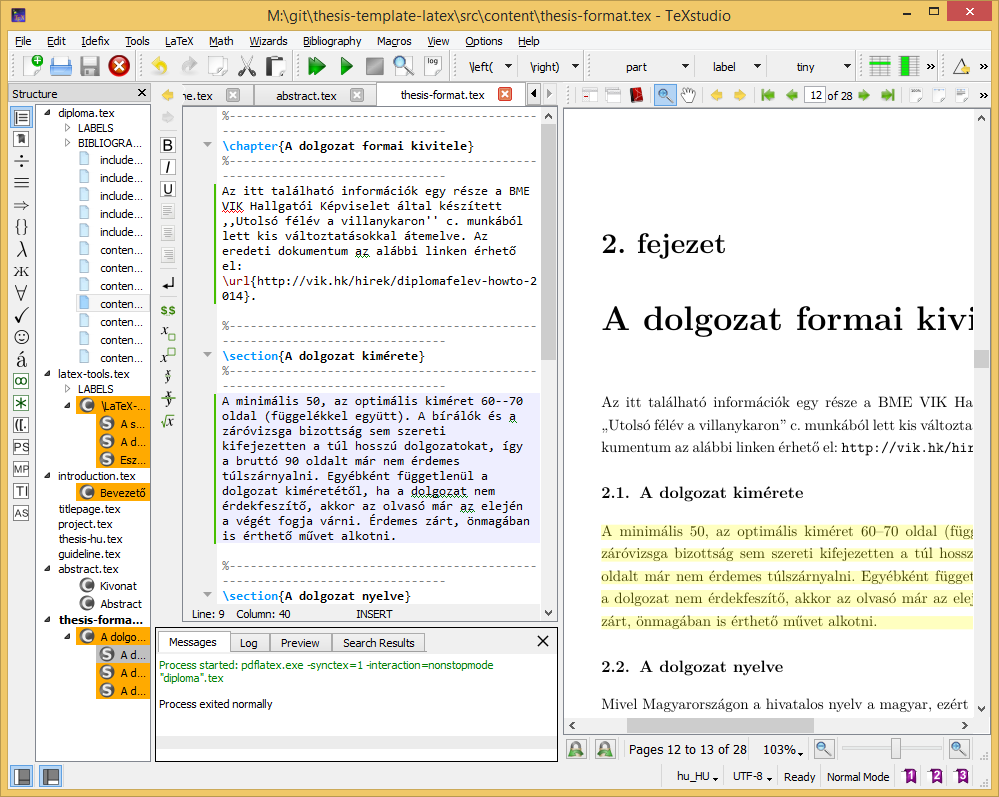
\includegraphics[width=150mm, keepaspectratio]{figures/TeXstudio.png}
\caption{A TeXstudio \LaTeX-szerkesztő.} 
\end{figure}

%----------------------------------------------------------------------------
\clearpage\section{Válasz az ,,Élet, a világmindenség, meg minden'' kérdésére}
%----------------------------------------------------------------------------
A Pitagorasz-tételből levezetve
\begin{align}
c^2=a^2+b^2=42.
\end{align}
A Faraday-indukciós törvényből levezetve
\begin{align}
\rot E=-\frac{dB}{dt}\hspace{1cm}\longrightarrow \hspace{1cm}
U_i=\oint\limits_\mathbf{L}{\mathbf{E}\mathbf{dl}}=-\frac{d}{dt}\int\limits_A{\mathbf{B}\mathbf{da}}=42.
\end{align}







%\label{page:last}
\end{document}
